% (C) Anders Kofod-Petersen
\documentclass[11pt, b5paper]{report}
\usepackage[english]{babel}						% Correct English hyphenation
\usepackage[utf8]{inputenc}						% Allow for non-English letters
\usepackage{graphicx}							% To include graphics
\usepackage{natbib}								% Correct citations
%\usepackage{fancyheadings}						% Nice header and footer
\usepackage[linktocpage,colorlinks]{hyperref}			% PDF hyperlink
\usepackage{geometry} 							% Better geometry
\usepackage{import}
\usepackage[toc,page]{appendix}
\usepackage{tabularx}
\usepackage[section]{placeins}
\usepackage{mathtools}
%\usepackage{amsmath}
\usepackage[]{algorithm2e}
%\usepackage[center]					% For cropping documents

% B5 (uncomment to convert to B5 format)
%\geometry{b5paper}

% Author
% Fill in here, and use commands in the text. 
\newcommand{\thesisAuthor}{Hanne Gunby and Susanne Gustavsen}
\newcommand{\thesisTitle}{Optimizing bus routes using AI-methods}
\newcommand{\thesisType}{Masters Thesis}
\newcommand{\thesisDate}{Spring 2014}

%Fancy headings
%\pagestyle{fancy}
%\pagestyle{fancyplain}
%\renewcommand{\chaptermark}[1]{\markboth{#1}{}}
%\renewcommand{\sectionmark}[1]{\markright{#1}{}}
%\lhead[\fancyplain{}{\thepage}]{\fancyplain{}{\let\uppercase\relax\leftmark}}
%\rhead[\fancyplain{}{\let\uppercase\relax\rightmark}]{\fancyplain{}{\thepage}}
%\chead[\fancyplain{}{}]{\fancyplain{}{}}
%\lfoot[\fancyplain{}{}]{\fancyplain{}{}}
%\cfoot[\fancyplain{}{}]{\fancyplain{}{}}
%\rfoot[\fancyplain{}{}]{\fancyplain{}{}}



\begin{document}

\pagenumbering{arabic}
%Title page (This is generate automatically from the commands above)
\begin{titlepage}
\noindent {\large \textbf{\thesisAuthor}}
\vspace{2cm}

\noindent {\Huge \thesisTitle}
\vspace{2cm}

\noindent \thesisType, \thesisDate 
\vspace{2cm}

\noindent Artificial Intelligence Group\\ Department of Computer and Information Science\\ Faculty of Information Technology, Mathematics and Electrical Engineering\\

\vfill

\begin{center}

\includegraphics[width=3cm]{assets/logo_ntnu_eng.pdf}

\end{center}

\end{titlepage}

\cleardoublepage

\section*{Abstract}
%The abstract is your sales pitch which encourages people to read your work but unlike sales it should be realistic with respect to the contributions of the work. It should include:
%\begin{itemize}
%\item the field of research
%\item a brief motivation for the work
%\item what the research topic is and
%\item the research approach(es) applied. 
%\item contributions
%\end{itemize}

%The abstract length should be roughly half a page of text --- without lists, tables or figures. 

The goal of this thesis is to optimize urban transit networks to make public transportation more convenient for passengers. A good transit network can reduce the number of vehicles on the road as people will favor public transport over their own transport, which will eventually reduce congestion and environmental emissions.

The Urban Transit Routing Problem (UTRP) deals with the creation of route networks.  UTRP is a complex and multiconstrained problem, in which creation of route networks can both be challenging and time consuming. Metaheuristics like swarm intelligence methods have proven to be effective for finding sufficient solutions to these types of NP-hard problems. In this contribution, a swarm inspired optimization system is designed and presented, aiming to create efficient solutions to the UTRP. The proposed system uses an ant colony approach with, unlike previous techniques, additional attributes inspired by bee colony optimization and particle swarm optimization. 

A structured literature review is conducted to synthesize the relevant primary studies, with a presentation and analysis of all retrieved studies.  Because metaheuristics require good initial parameters to solve concrete problems optimally, a thorough review and justification of each selected parameter is documented. This documentation will contribute in providing a starting point for potential future research. A comparison against a standard ant colony optimization (ACO) implementation is performed to demonstrate whether the proposed system improves the standard ACO. To demonstrate the performance of the proposed system, obtained results are compared on the basis of Mandl's benchmark problem, which is a widely investigated and accepted benchmark problem. The proposed system is also tested on larger networks, more similar to real transit networks, to validate whether the proposed system supports larger networks as input. This thesis will also report how the usage of the graph database Neo4j has affected the performance and quality of the proposed solution. 

The proposed system performs better than the standard ACO method. Comparison of obtained results with other published results is promising, especially regarding the average traveling time per transit users. 

\section*{Sammendrag}

Urban Transit Routing Problemer (UTRP) tilhører en klasse av NP-harde optimeringsproblemer, der den optimale løsningen ikke nødvendigvis er mulig å finne. UTRP omhandler konstruksjon av rutenettverk for kollektivtransport. Det er et komplekst og multi begrenset problem, der konstruksjon av rutenett kan være både tidkrevende og utfordrende. Metaheuristiske metoder som sverm intelligens har vist seg å være effektive for å finne tilstrekkelige løsninger på NP-harde problemer. I dette bidraget, er et sverm inspirert optimalisering system derfor utformet og presentert, med sikte på å skape effektive løsninger til UTRP. Det foreslåtte systemet bruker en ant colony tilnærming som, i motsetning til tidligere løsninger, har tilleggsattributter inspirert av bee colony optimization og particle swarm optimization. Resultatene er sammenlignet på basis av Mandl benchmark problem, som er et allment akseptert benchmark problem i  relevant litteratur. Sammenligning av oppnådde resultater med andre publiserte resultater er lovende, spesielt med tanke på gjennomsnittlig reisetid per reisende.

\clearpage
\section*{Preface}
%The preface includes the facts - what type of project, where it is conducted, who supervised and any acknowledgments you wish to give.

This document and its associated source-code is the end product of the Masters Thesis of Hanne Gunby and Susanne Gustavsen at the Norwegian University of Science and Technology (NTNU). 
%\newline
%\newline


\section*{Acknowledgments}

Thanks to Anders Kofod-Petersen and Jo Skjermo for valuable feedback and advice throughout the process.

Thanks to Agnar Aamodt for always keeping his door open and answering questions.

Thanks to Torkil Rein Gustavsen for introducing us to Cloud Computing.

Thanks to friends and fellow students for helpful discussions.

Finally, thanks to our family for endless love and support.
\clearpage

%content
\listoftables
\listoffigures
\tableofcontents

\chapter{Introduction}
\label{introduction}
AtB is responsible for planning, ordering and marketing public transport throughout Sør-Trøndelag county.


\section{Background and Motivation}

Trondheim and neighboring municipalities are among the areas with the greatest population growth in Norway \citep{website:miljopakken}. More people means more traffic, and without action will congestion and environmental problems in these urban areas continue to increase every year. 

Private transportation has many advantages for the citizens compared to the public ones. The citizens do not have to wait for a vehicle or change vehicles during a trip, and it is often more convenient. But private transportation has a lot of negative issues, such as traffic jams and increased travel times, which leads to increased air pollution, noise and accidents. 

Having efficient public transportation systems can substantially reduce negative effects of the private transportation networks. The environment package \citep{website:miljopakken} for transport in Trondheim aims to provide better road networks and public transportation. With this they hope to achieve lower emissions, shorter traffic jams and less traffic noise. An inadequately designed transit network can cause very long waiting times and increase uncertainty in bus arriving time, resulting in less people taking use of the service. Therefore, public transportation systems should be improved by providing better travel services, and inform the public about them, in order to convince more people to travel with it instead of using their own car. 

\citet{website:atb} is responsible for planning the public transport throughout Sør-Trøndelag County, and bus services comprise the major component of the public transportation system. From a meeting with AtB we learned that the current solution of AtB consists of an experience based route network, where no common methodology is used, and where all bus route networks and schedules are designed manually. As a result, the efficiency of the resulting networks is highly dependent of the designers expedience and his / hers knowledge of existing resource constraints and transportation demands. The manual attempts to provide an acceptable solution to the urban routing and scheduling problems are not able to solve these large network problems efficient.

Satisfying all customer needs in addition to keeping all operator costs in check is really difficult to achieve. The problem of designing the optimal set of routes for a fleet of vehicles, in order to serve a given set of customers, is referred to the vehicle routing problem (VRP). The urban transit network problem(UTNDP) is an example of the broader optimization problem VRP, and is the problem of designing urban transit routes and schedules. The two major components of the UTNDP are the urban transit routing problem(UTRP) and the urban transit scheduling problem (UTSP). \citep{fan09}.
UTRP involves the development of efficient transit routes on an existing transit network, with predefined pick-up/drop-off point (e.g bus routes), and UTSP is assigning the schedules for the passengers carrying vehicles. In practice, the two phases are usually implemented sequentially, with the routes determined in advance of the schedules. 


%TODO: Hanne: fortelle kort om hvorfor swarm intelligence er interessant. 












\section{Goal and Research Questions}
%TODO: skrive et mer utfyllende avsnitt
\textbf{Goal:}
\begin{itemize}
\item \label{itm:goal} Increase the number of public transportation passengers by making urban transit networks more efficient.
\end{itemize}
\textbf{Research Questions:}
\begin{enumerate}[label=\textbf{\arabic*})]
\item \label{itm:1}
    \begin{enumerate}
    \item \label{itm:1a} \textbf{Is swarm intelligence methods suitable for the vehicle routing problem?}\newline
    This research question concerns whether or not swarm intelligence methods are suitable for solving vehicle routing problems. 
    \item \label{itm:1b} \textbf{What is the state-of-the-art in solving vehicle routing problems using swarm intelligence methods?}\newline
    This research question is dependent on the question above. If swarm intelligence methods in fact are suitable for solving vehicle routing problems we want to establish what the state-of-the-art is. 
    \item \label{itm:1c} \textbf{What changes have been done to the classical swarm intelligence-methods to improve them?}\newline
    After we have established the state-of-the art, we want to study what changes that have been done to the classical swarm intelligence methods to improve them. This will help us identify what changes that have proven to be successful/unsuccessful in the past, and allow us to get inspiration from this when designing our own model.  
    \item \label{itm:1d}\textbf{Have there been any attempts to combine different swarm intelligence-methods?} \newline
    Because we are motivated by creating a solution that combines different attributes from different swarm intelligence-methods, this question will help us establish if there have been conducted research that tries exactly that. 
	\end{enumerate}
    Research Question 1 as a whole will be answered after a Structured Literature Review, and Research Questions 2 and 3 are created based on the answers. 
\item
    \begin{enumerate}
    \item \label{itm:2a} Is it efficient to add attributes from other swarm intelligence-methods in order to improve the ant colony optimization algorithm?
    \item \label{itm:2b1} How does the proposed method perform compared to methods published in literature?
    \item \label{itm:2c} Is it possible to apply the proposed algorithm to optimize urban transit routes in real urban cities?
    \end{enumerate}
\item
	\begin{enumerate}
    \item \label{itm:3a} Have graph databases been employed in combination with the vehicle routing problem and swarm intelligence?
	\item \label{itm:3b} What are the potential advantages and disadvantages of using a graph database in our implementation?
    \end{enumerate}
\end{enumerate}
\section{Research methods}

%What methodology will you apply to address the goals: theoretic/analytic, model/abstraction
%or design/experiment? This section will describe the research methodology applied
%and the reason for this choice of research methodology.

In this thesis, two research methods are applied. The first research method used is a structured literature review, introduced by \citep{kofod2014}. This research is conducted in order to establish the state-of-the-art of using swarm intelligence methods and graph databases to solve Vehicle Routing Problems. The results of the final synthesis are presented as the related work that further forms the basis for the proposed problem statement. 

The second research method is the design and development of the proposed system. Experiments comparing the proposed system to a generic ACO algorithm and several published methods are conducted. To ensure a sufficient comparison basis, the proposed system use a well-known benchmark problem.  

The proposed system also attempts to solve larger problems than the benchmark problem described above. By larger problems, we mean a network with a realistic number of bus stops, roads and routes in the route set. This will establish whether the proposed system supports larger networks, which further allow us to discuss the possible usability in a real urban city. 

For all the experiments, numeric values of established performance criteria, including average travel time, is presented. These values are further used to discuss the performance of the proposed system

%The comparison will be based on the numeric values of well-established performance criteria, such as average travel time experienced by each passenger.

%Experiments comparing the proposed system to other methods described in literature will be conducted. This is done

%In order to answer \vref{itm:RQ1} a Structured Literature Review, as described by \citep{kofod2014}, is conducted. This is done to ensure that we are able to draw valid conclusions about what the state-of-the-art is. The results of the final synthesis is described in Related Work, and this is the basis for the problem statement.

%The research method that is used in order to answer \vref{itm:RQ2} and \vref{itm:RQ3}, is designing the proposed system and conducting relevant experiments. 

%In order to test whether or not the added attributes from other swarm intelligence algorithms is efficient, the performance of the proposed algorithm and generic ACO algorithm is compared. 

%To establish how the proposed system performs compared to other methods described in literature, experiments solving a well-known benchmark problem with the proposed system is conducted. 

%In order to test if the proposed system is applicable for optimizing the transit routes in large urban cities, the proposed system will be tested with larger networks as input. 



\section{Thesis Overview}

%\begin{itemize}
%\item What does this thesis contain
%\item Give results in a general way
%\end{itemize}

%This section provides the reader with an overview of what is coming in the next
%chapters. You want to say more than what is explicit in the chapter name, if
%possible, but still keep the description short and to the point.

Chapter 2 sets the context for this thesis. It starts by discussing the domain swarm intelligence in Section \ref{sec:swarmIntelligence}, and includes theory about Ant Colony Optimization (ACO), Bee Colony Optimization (BCO) and Particle Swarm Optimization (PSO). In Section \ref{sec:VRP} the Vehicle Routing Problem (VRP) is described, along with the Urban Transit Network Design Problem, which is a subproblem of the VRP. Section \ref{sec:graphdb} is describes graph theory and puts it in context with graph databases. The graph database ``Neo4j'' is also presented. 
\newline
\newline
Chapter 3 describes the preparatory research done in order to develop the proposed method. Section \ref{sec:definingResearchTopic} defines the research topic used in order to guide the Structured Literature Review\citep{kofod2014}, which further is described in Section \ref{sec:structuredLiteratureReview}. Section \ref{sec:relatedWork} describes and discusses related work and will at the end answer \ref{itm:RQ1}. Finally, in Section \ref{subsec:problemStatement} the problem statement is proposed.  
\newline
\newline


\chapter{Background and Motivation}
\label{backgroundAndMotivation}
 \citet{website:atb} is responsible for planning the public transport throughout Sør-Trøndelag County, and bus services comprise the major component of the public transportation system. From a meeting with AtB we learned that the current solution of AtB consists of an experience based route network, where no common methodology is used, and where all bus route networks and schedules are designed manually. As a result, the efficiency of the resulting networks is highly dependent of the designers expedience and his / hers knowledge of existing resource constraints and transportation demands.

 Satisfying all customer needs, and keeping all operator costs in check, is really difficult to achieve \citep{kechagiopoulos14}. Operator costs mainly refer to the total number of buses, total bus running distance and the total operation hours. A minimum trip time, amount of transitions, and a not too crowded bus (customers can tolerate standing in 15 minutes ) are among the most important factors that determine the passengers choice of public transit, AtB experiences.  
 \textit{The main concern of bus companies is maximizing its profits, while the main concern of the government is to fulfill all needs of traveling in public} \citep{kechagiopoulos14}. The manual attempts to provide an acceptable solution this problem are not able to solve these large network problems efficiently \citep{kechagiopoulos14}. 
\section{Vehicle Routing Problem }

The Vehicle Routing Problem (VRP) was first introduced by \citet{dantzig59} and is a generic name given to a broad class of optimization problems. It can be described as the task of designing the optimal set of routes for a fleet of vehicles, in order to serve a given set of customers. The problem involves making deliveries to a set of customers with known demands on routes originating and terminating at one or more depots. The objective of any routing problem is usually the minimization of costs ( e.g. reducing the route lengths, the number of vehicles, or minimize the total route cost) . 

Routing problems are represented as a road network by relevant locations in a graph, and this graph consist of a set of nodes an a set of edges, G = (V,E). Nodes are directly connected by some edge, and it can be an undirected or a directed network. 
%They can be distinguished according to the type of requests that need to be serviced, that is either arc-based and node-based routing problems. The vehicle routing problem (VRP) is a node based routing problem, as these problems arise if customers are located at nodes so that vehicles remain at the same position while servicing a customer request \citep{vehiclerouting}. ) 
%The structure of a network can be a matrix formulation, aij, where i and j are nodes. 
% adjacency matrix aij(1: arc 0: no arc) or incidence matric bij ( -1 arc j starts at vertex i, 0: arc j neither starts nor ends at vertex i. -1: arc j ends at vertex i).
%A connected graph means it is complete, and this means it contains as many edges as possible, without having any edge more than once. 

\subsection{Urban Transit Network Design Problem}

The problem of designing urban transit routes and schedules is called the urban transit network problem (UTNDP), and is a sub-problem of the VRP. The aim is to design efficient urban transit routes and schedules on an existing transit network with predefined pick-up and drop-off points, such as bus routes, while adhering to practical constraints (e.g maximum and minimum length for each route, a limited number of stops, a connected route set). The two major components of UTNDP is called the urban transit routing problem (UTRP) and the urban transit scheduling problem (UTSP):

\begin{itemize}
\item UTRP is the task of developing a set of routes on an existing urban transit network, following certain constraints. It can be defined as the \textit{physical} design of the UTNDP \citep{fan09}. 

%TODO: Denne må gjøres om til å stå route set ikke tour plan
In a transit network, neighboring nodes (bus stops) are linked by an arc or edge. Each step in a tour, traveling from one node to the next, is called a route, and a route will consist of several nodes connected by edges to form a path. A route set consists of several routes combined. When all the routes in a route set are superimposed / layered, it will a form a route network, and is also denoted as the solution of the considered problem. The generation of a route set is defined by the objective function, and assigns a specific objective function value to each solution. The goal is to find the optimal solution; the ones with the best objective function among all feasible solutions \citep{vehiclerouting}. A route network should contain all the nodes, but may not contain all the edges present in the original transit network. The criteria for a good route set includes that the entire transit demand is served, and a large percentage of this demand is served through direct connections. In addition, the average travel time per transit user should be as low as possible. 

\item UTSP involves the development of schedules, arrival and department times, for the public vehicles, to travel along predefined routes. It can also be defined as the \textit{operational} design of the UTNDP \citep{fan09}. 
The contents of the schedule involves minimizing the time a passenger has to wait at each node (bus stop), following certain constraints, such as limited fleet size and bus capacity.  The total waiting time includes the waiting time at their origin, in addition to the sum of transferring time.

UTRP and UTSP are usually implemented sequentially, because the development of routes should be completed before the development of schedules. 
\end{itemize}

There are some difficulties in solving the UTNDP. First of all, the UTNDP is an NP-hard problem due to the need to search for optimal solutions from a large number of possible solutions. Some of the constraints can be difficult to model and satisfy, as the feasibility of the tour plan needs to be ensured, which can involve a significant number of computations. Travel demand can be difficult to get hold of and can be different at every hour of the day, and designs will therefore be flawed if the data is of poor quality.  

%\subsubsection{Difficulties in Solving the UTNDP}
%TODO: skrive om / flette dette inn i motivation? 
%There are some difficulties in solving the UTNDP. First of all, the UTNDP is an NP-hard problem due to the need to search for optimal solutions from a large number of possible solutions. Some of the constraints can be difficult to model and satisfy, as the feasibility of the tour plan needs to be ensured, which can involve a significant number of computations. Parts of the solutions are independent, because a performance of a route is dependent on the other routes in the tour plan. Travel demand can be difficult to get hold of and can be different at every hour of the day, and designs will therefore be flawed if the data is of poor quality. In addition, passengers can become confused or dissatisfied if there are to many changes to travel routes different times of day, AtB says. The ideal situation would be to solve UTNDP in one go, and produce a route network and an associated set of vehicle frequencies simultaneously. But in practice, the nature of a route network means that, once established, it is much more stable and difficult to change than a vehicle schedule. Since travel demand varies, it is easy to schedule more buses at busy times. The level of service requirements is sensitive factors (passenger flow, weather and road conditions), and needs to be adjusted to different situations. Therefore, the quality of the network design may be adversely influenced if transit route network and frequencies are simultaneously optimized. 





\section{Swarm Intelligence}

Swarm behavior is found in many different species in nature, including fish schools and flocks of birds. Many of the species that practice swarm behavior does this because of a biological need to stay together. An example of this is that predators usually attacks one individual, and not an entire flock. This swarm behavior is also found in social insects like ants, wasps, bees and termites. They collaborate on tasks including building nests, gather food and organizing production. These social insect colonies have shown us that simple organisms can perform complex tasks by interacting with each other. The colonies are highly distributed and self-organized, and they adapt well to changes in the environment. Swarm intelligence \citep{beni89} is a branch of artificial intelligence that is strongly influenced by the swarm behavior found i nature, and it tries to adapt these characteristics in intelligent computer systems.

\subsection{Ant Colony Optimization}
In nature ants have proven to be extremely capable of finding an optimal or close to optimal route from the nest to a food source \citep{deneubourg90}. Ants communicate by leaving a pheromone trail that other ants are capable of smelling and follow by a certain probability. Most ant species leave a pheromone trail when retuning to the nest from an important food source, and the ants who decides to follow the same path also leave behind a pheromone trail. The more pheromone units on the trail (i.e. the more ants who choose the given path), the greater the probability the other ants will chose it. Because pheromone disappear over time, shorter paths will be favored over longer paths simply because shorter paths (usually) takes shorter time, and thus will have more pheromone units. 

Ant Colony Optimization (ACO) is a class of graph representation based metaheuristic algorithms designed to optimize routing problems. The first description of an ACO algorithm, called Ant System (AS), was initially proposed by \citet{dorigo96}. The AS strategy developed by Dorigo tries to simulate the behavior of real ants, but he adds several artificial characteristics including visibility, memory and discrete time. \citet{nanda11} described a generic implementation of the algorithm as follows: \\

\begin{algorithm}[H]
 initialize\;
 \While{stop criteria are not met}{
  \ForAll{ants a in A}{
   position a in StartNode
  }
  \Repeat{every ant has a solution}{
   \ForAll{ants a in A}{
    choose nextNode\\* 
    $pheromone_{(currentNode,nextNode)}+=update$
   }
  }
  \ForAll{edges e in B}{
   $pheromone_e += deposit$
  }
  \ForAll{edges e in E}{
   $pheromone_e -= evaporation$
  }
 }
 \caption{Generic Ant Colony Optimization Algorithm}
\end{algorithm}

The idea of ACO algorithms is to create a decentralized system with multiple agents. The agents influence each others decisions using pheromones. In the beginning, before any distinct pheromone trail is laid, the ants choices are random and thus they perform a broad search in the environment. This randomness will decrease over time as the pheromone trails becomes more distinct. The literature describes many different algorithms that can be classified as ACO algorithms \citep{salehi-nezhad07,tripathi09,jiang10, dias14}, and most of authors describes artificial ants with additional features to those found in nature, including vision and memory. The addition of features is typically done to increase the performance of the algorithm and reduce some of the randomness in the beginning.  

%TODO: SKRIVE OM ACO I RUTEOPTIMALISERING! 

\subsection{Bee Colony Optimization}
As described in \citet{lucic03}, bees are capable of performing a variety of complex tasks. One of these tasks are the collection and processing of nectar, which may be considered as extremely organized. The idea is that a bee that leaves the hive to gather nectar, flies to the hives so-called dance floor. The bees that have already found a good food source performs a ``dance'' at the dance floor to advertise that they have found a satisfying source of food. The bee that just came from the hive chooses one of the dancing bees and flies with it to its food source. As stated in \citet{lucic03} the mechanism of deciding which bee to follow is not well understood, but it is considered that ``the recruitment among bees is always a function of the quality of the food source''. After the bee has gathered and returned the food to the hive, the bee has three options\citep{lucic03}:

\begin{enumerate}
  \item It can abandon the food source and return to the dance floor, and again become an uncommitted follower
  \item It can continue to gather nectar from the food source without recruiting nestmates
  \item It can return to the dance floor and dance, and thus recruit nestmates before returning to the food source
\end{enumerate}

Bee Colony Optimization (BCO) is metaheuristic methods, that like ACO, aims to create a decentralized optimization system with multiple agents, based on graph representation. The idea is to apply the collective intelligence of the food gathering process to an optimization system. Like a typical ACO algorithm, a typical BCO algorithm is inspired by the way bees acts in nature, but some of the features of natural bees are added to and removed from the artificial bee. \citet{nikolic14} describes a BCO algorithm where the artificial bee only has two options after returning from a ``food source'': (1) abandon or (2) recruit. \citet{lucic03} gives the artificial bees attributes such as memory and perfect knowledge about the quantity of nectar collected by other bees. Modifications like these can make the algorithms more efficient, and thus more suitable of performing complex combinatorial problems, like the Traveling Salesman Problem. 


\subsection{Particle Swarm Optimization}
%[TODO]: Skrive om PSO
% http://ieeexplore.ieee.org/stamp/stamp.jsp?tp=&arnumber=785511
As reported in \citet{referanse} Particle Swarm Optimization (PSO) was first introduced by Eberhart and Kennedy in 1995. PSO is inspired by the social behavior of flocks (such as flocks of birds) and schools (such as fish schools), and the idea is to update the population of individuals according to the individual's own experience and its companions' experience. This is unlike other evolutionary computational algorithms, like Genetic Algorithms, that uses evolutionary operators to manipulate the individuals. The basic concept is that each individual flies (or swims) with a certain velocity, and that this velocity is dynamically adjusted based on the experience. \citet{referanse}

%TODO: Skrive om fordeler og ulemper
%TODO: Kanskje finne en algoritme
%TODO: Skrive om PSO i litteraturen



\section{Graph Databases}

Graphs are one of the most efficient and natural way of working with data. Formally speaking a graph is just a collection of vertices and edges. The term \textit{graph theory} been used in centuries, and was first introduced by the Swiss mathematician Leonard Euler (1707-1783) when he in 1736 proved that there does not exist a closed walk that crossed exactly once each of the seven bridges of the river Pregel in Köningsberg, now called Kaliningrad\citep{alexanderson06}. Figure \ref{fig:7bridgesEuler} shows Eulers original drawings from his paper written in 1736 \citep{euler1741} of the bridges in Köningsberg. 

\begin{figure}[H]
  \centering
  \includegraphics[width=4in]{assets/7bridges-euler.png}
  \caption{Eulers original drawing of the Seven Bridges of Köningsberg} 
  \label{fig:7bridgesEuler}
\end{figure}

Based on the solution of the ``Seven Bridges of Köningsberg''-problem, Euler presented a theorem that states that if the graph is planar and connected, and if \textit{v} is the number of vertices, \textit{e} is the number of edges and \textit{f} is the number of faces (regions between edges of a plane graph that does not have any edges in it), then 
\newline
\newline
\centerline{$v-e+f=2$}
\newline
\newline
This means, with respect to the ``Seven Bridges of Köningsberg''-problem, that if it does not exists a path in the graph that lets you visit every node using every edge exactly once, the sum will not be 2. We have illustrated the bridges in Köningsberg as a graph in figure \ref{fig:7bridgesIllustration} and simplified the illustration in figure \ref{fig:7bridgesSimplification}. We see that the graph consists of 4 vertices, 7 edges and 4 faces. The faces are specified with numbers 1-4 in figure \ref{fig:7bridgesSimplification}. If we use the theorem described above we see that $4-7+4\neq2$, which is consistent with Eulers proof from 1736. 

\begin{figure}[H]
  \centering
  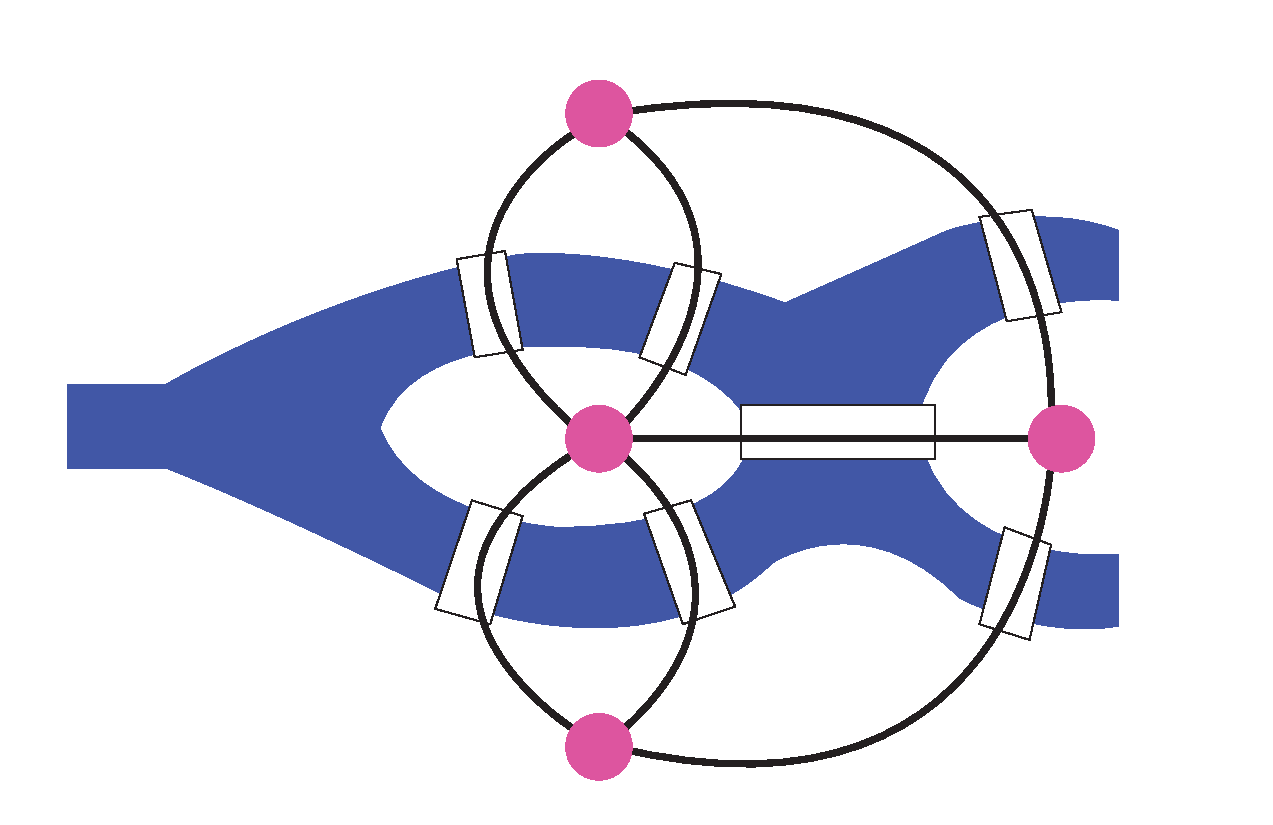
\includegraphics[width=4in]{assets/7bridges.pdf}
  \caption{Illustration of the Seven Bridges of Köningsberg as a graph} 
  \label{fig:7bridgesIllustration}
\end{figure}

\begin{figure}[H]
  \centering
  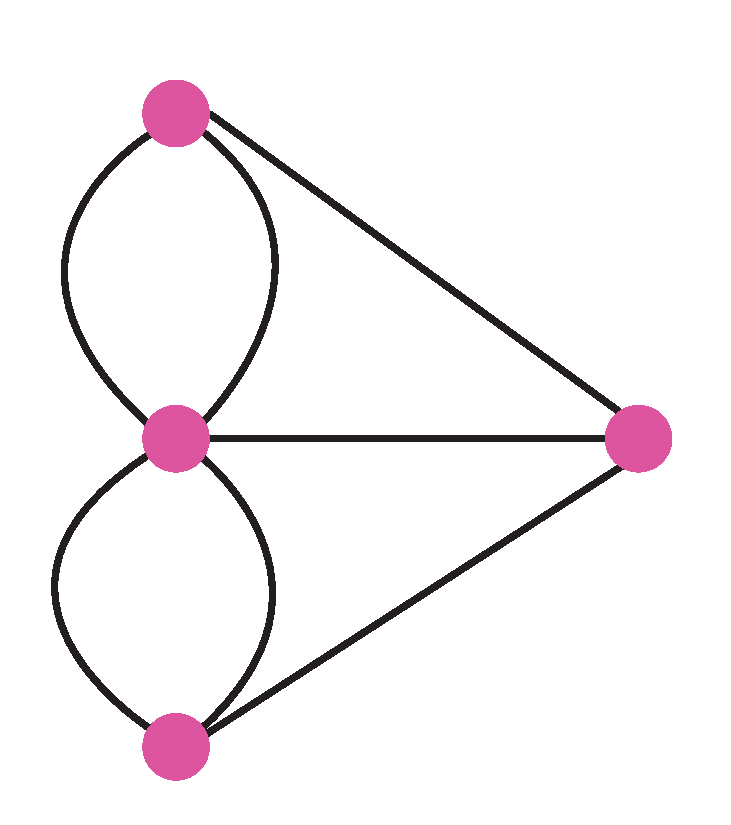
\includegraphics[width=2in]{assets/7bridges2.pdf}
  \caption{The simplified graph of the Seven Bridges of Köningsberg} 
  \label{fig:7bridgesSimplification}
\end{figure}

%Graph theory is a mature and well-understood field of study concerning the nature of
%networks (or from our point of view, connected data)\citep{robinson13}. 

Graph databases consists of nodes, edges, and properties to represent and store data. Nodes represent entities, such as people, accounts and bus stops,(each node knows its adjacent nodes) properties are relevant information that relate to the nodes, and edges are the lines that connect the nodes and properties, defining the relationship between them. Most of the information is stored in the edges, for instance the travel time or travel demand between to nodes. 

A graph database management system (henceforth, a graph database) is an online database management system with Create, Read, Update, and Delete (CRUD) methods that expose a graph data model. 

It uses graph structures for semantic queries. It is a storage system where every element contains a direct pointer to its neighbor elements and no index lookups are necessary. 

\par %Skrives om litt

Relational and NOSQL databases lack relationships \citep{robinson13}. Compared to relational databases, are graph databases often faster for associative data sets[Wikipedia:P], and map more directly to the structure of object-oriented applications. They can scale more naturally to large data sets as they do not typically require extensive join operations. As they depend less on a inflexible schema, they are more suitable to manage changing data with evolving schema's.

\par
Graph databases are a powerful tool for graph-like queries, for instance computing the shortest path between to nodes in the graph!!! Other graph-like queries can be performed over a graph database in a natural way (for example graph's diameter computations or community detection).

%Geospatial is the original graph use case: Euler solved the Seven Bridges of Königsberg problem by positing a mathematical theorem that later came to form the basis of graph theory. Geospatial applications of graph databases range from calculating routes between locations in an abstract network such as a road or rail network, airspace network, or logistical network to spatial operations such as find all points of interest in a bounded area, find the center of a region, and calculate the intersection between two or more regions. \citep{neo13}
%Geospatial operations depend upon specific data structures, ranging from simple weighted and directed relationships, through to spatial indexes, such as R-Trees, which represent multidimensional properties using tree data structures. As indexes, these data structures naturally take the form of a graph, typically hierarchical in form, and as such they are a good fit for a graph database. Because of the schema-free nature of graph databases, geospatial data can reside in the database beside other kinds of data—social network data, for example—allowing for complex multidimensional querying across several domains. Geospatial applications of graph databases are particularly relevant in the areas of telecommunications, logistics, travel, timetabling, and route planning \citep{neo13}

\par

\textit{Denne er foreløpig kopiert fra Wikipedia: }%Skrives om 
Compared with relational databases, graph databases are often faster for associative data sets[citation needed], and map more directly to the structure of object-oriented applications. They can scale more naturally to large data sets as they do not typically require expensive join operations. As they depend less on a rigid schema, they are more suitable to manage ad hoc and changing data with evolving schema's. Conversely, relational databases are typically faster at performing the same operation on large numbers of data elements.
Graph databases are a powerful tool for graph-like queries, for example computing the shortest path between two nodes in the graph. Other graph-like queries can be performed over a graph database in a natural way (for example graph's diameter computations or community detection).

\subsection{Neo4j}
Neo4J \citep{website:neo4j} is a native graph database, native graph storage that is optimized and designed for
storing and managing graphs.

and is a success way to store a transport graph. It is known for extremely fast traversals of relationships. Neo4J can be easily constructed to a transit network. It is fast finding shortest path (by Dijkstra's algorithm), and it is easy to change the database via the REST API. 

Neo4J is a highly scalable open source graph database that supports ACID, has high-availability clustering for enterprise deployments, and comes with a web-based administration tool that includes full transaction support and visual node-link graph explorer. Neo4j is accessible from most programming languages using its built-in REST web API interface. Neo4j is the most popular graph database in use today.[10]

Advantages:
\begin{itemize} 
\item Flexibility: model, develop and visualize the world as you experience it. Its simply nodes and relationships. 
\item Performance: Hyper-connectivity at speed. 
\item Scalability: Scales up and out, supporting tens of billions of nodes and relationships, and hundred of thousands of ACID transactions per seconds. 
\item Speed: Able to search trough millions of connections per second, with real time queries that stay fast even as your database grows. 
\end{itemize}

\subsubsection{Dijkstra's algorithm}
Dijkstra  is used  by Neo4j to find the shortest path between two nodes in the graph. Dijkstra’s algorithm is mature, having been published in 1956, and thereafter widely studied and optimized by computer scientists.\citep{neo13}. Dijkstra’s algorithm is quite efficient because it computes only the lengths of a relatively small subset of the possible paths through the graph. Dijkstra is often used to find real-world shortest paths (e.g., for navigation). It behaves as follows:
\begin{enumerate}
\item Pick the start and end nodes, and add the start node to the set of solved nodes (that is, the set of nodes with known shortest path from the start node) with value 0 (the start node is by definition 0 path length away from itself).
\item From the starting node, traverse breadth-first to the nearest neighbors and record the path length against each neighbor node.
\item Take the shortest path to one of these neighbors (picking arbitrarily in the case of ties) and mark that node as solved, because we now know the shortest path from the start node to this neighbor.
\item From the set of solved nodes, visit the nearest neighbors (notice the breath-first progression) and record the path lengths from the start node against these new neighbors. Don’t visit any neighboring nodes that have already been solved, because we know the shortest paths to them already.
\item Repeat steps 3 and 4 until the destination node has been marked solved.
\end{enumerate}


%\begin{itemize}
%\item Native graph database. 
%\item Property graph. 
%\item Made for real time queries. 
%\item Really fast traversals of relations.
%\item Neo4J has an API that supports traversing - finding shortest path - can weight edges, nodes -
%\end{itemize}
%//en korteste vei mellom n og m men max lengde 3
%match p = shortestPath ( (n) - [*...3]--(m)) return p
%(Vekte kanter: Neo44J har et API som støtter traversering, Dijkstras er innebyd ++ som lar deg vekte kanter - hva er raskeste vei ++)

%Neo4J can be used to evaluate routes after the ants have created route sets.
\section{Motivation}

Trondheim and neighboring municipalities are among the areas with the greatest population growth in Norway \citep{website:miljopakken}. More people means more traffic, and without action will congestion and environmental problems increase every year. 

Private transportation have many advantages for the citizens compared to the public ones. They do not have to wait for a vehicle at the beginning of a trip, change vehicles during the trip, and it is often more convenient. The negative issues of private transportation, such as traffic jams and increased travel times, means increased air pollution, noise and accidents. 

Having efficient public transportation systems can substantially reduce negative effects of private transportation networks 
\citep{kechagiopoulos13} . The environment package \citep{website:miljopakken} for transport in Trondheim involves providing better road networks and public transport. With this they hope to achieve lower emissions, shorter traffic jams and less traffic noise. Inadequately designed transit network can cause very long waiting times and increase uncertainty in bus arriving time \citep{nikolic14}. Therefore, public transportation systems should be improved by providing better travel services, and inform the public about them, in order to convince more people to travel with it instead of using their own car. 

 \citet{website:atb} is responsible for planning the public transport throughout Sør-Trøndelag County. \textit{Among public transportation alternatives, “bus” has specific attractive features. These are flexible routes, medium capacity, low cost (of capital and running), easy implementation, flexible fleet size (easy to expand or contract this size), and use of existing facilities (roads and streets).} In Trondheim, bus services comprise the major component of public transportation system. From a meeting with AtB we learned that the current solution of AtB consists of an experience based route network, where no common methodology is used, and where all bus route networks and schedules are designed manually. As a result, the efficiency of the resulting networks is highly dependent of the designers expedience and his / hers knowledge of existing resource constraints and transportation demands. Satisfying all customer needs, and keeping all operator costs in check, is really difficult to achieve \citep{kechagiopoulos13}. Operator costs mainly refer to the total number of buses, total bus running distance and the total operation hours. A minimum trip time, amount of transitions, and a not too crowded bus (customers can tolerate standing in 15 minutes ) are among the most important factors that determine the passengers choice of public transit, AtB experiences.  \textit{The main concern of bus companies is maximizing its profits, while the main concern of the government is to fulfill all needs of traveling in public} \citep{kechagiopoulos13}. The manual attempts to provide an acceptable solution the Vehicle Routing Problem are not able to solve these large network problems efficiently \citep{kechagiopoulos13}. 

 \textit{The number of journal publications on Vehicle Routing Problems has steadily increased over the years. This is because of the progress in computational resources has opened new possibilities for modeling more complex routing problems. New arising real-world applications provide inspiration for developing new approaches for coordinating complex transportation processes.}  \citep{vehiclerouting}




















\chapter{The Model}
\label{theModel}
Here you will present the architecture or model that you have chosen and that is (or will be) implemented in your work. Note that putting algorithms in your report is not desirable but in certain cases these might be placed in the appendix. Code further be avoided in the report itself but may be delivered in the fashion requested by the supervisor or, in the case of masters delivery, submitted as additional documents. 

\textit{This is the main structure of what you built.
- Not at code level, but you can include pseudocode.
Explain the system in a way the reader understands it.
Include diagrams and the algorithms used.}

TODO: Skrive om hvorfor vi har valgt å kode i java. speed, vi kan det best, (ne04j) ++

\section{Input Data}

%TODO: Referanser til hvor vi lastet ned dataen

We have designed and implemented a method to produce a realistic transit network based on the data from Mandl \citep{mandl79}. The transportation time on each edge is given, and the transportation demand is assumed to be known and constant. 

To do this we have constructed a transit network, including edges and nodes, based on the data set we have downloaded from \
citet{fan09}, which consist of text files:




\begin{table}[h!]

    \begin{tabular}{|l|lr|}

 	\hline
 	~ & x & y \\
 	\hline
    1 & 1 & 9 \\
    2 & 3 & 8 \\
    3 & 4.5 & 7.75 \\
    4 & 2.75 & 6.2 \\
    5 & 0.8 & 6.6 \\
    6 & 4.6 & 6 \\
    7 & 7 & 4.5 \\
    8 & 5.5 & 5 \\
    9 & 8.5 & 6.8 \\
    10 & 5.8 & 2.25 \\
    11 & 3.8 & 2.25 \\
    12 & 1.3 & 3.5 \\
	13 & 5.25 & 1 \\
	14 & 6.7 & 1.75 \\
	15 & 6.75 & 5.8 \\
	\hline
    \end{tabular}
    \caption {Mandl Coordinates}
\textit{The MandlCoord.txt file includes 15 lines, with the (x,y) coordinates of the 15 nodes. These coordinates was not supplied in Mandl's literature, so these are copied from \citet{fan09} and are approximate for the picture to be drawn.}
\end{table}


\begin{table}[h!]
    \begin{tabular}{|l|lllllllllllllll|}
    \hline
    ~ & 1       & 2        &  3    &   4     &  5     &  6      & 7      &  8     & 9      & 10      & 11     & 12         &  13     & 14       &  15  \\
    \hline
    1 & 0       & 8        &  Inf    &   Inf     &  Inf     &  Inf      & Inf      &  Inf     & Inf      & Inf      & Inf     & Inf         &  Inf     & Inf       &  Inf  \\
    2 &8       & 0        & 2       &  3        &  6       &  Inf      & Inf      & Inf      & Inf      & Inf      & Inf     & Inf         &  Inf     &  Inf      &  Inf  \\
    3 & Inf     &  2       &  0      &  Inf      & Inf      &  3        &  Inf     &  Inf     & Inf      &  Inf     & Inf     &  Inf        &  Inf     &   Inf     & Inf   \\
    4 & Inf     &  3       &  Inf    &  0        & 4        & 4         & Inf      &  Inf     &  Inf     & Inf      & Inf     & 10          &  Inf     &  Inf      &  Inf  \\
    5 & Inf     &   6      &   Inf   &    4      &   0      & Inf       &  Inf     &  Inf     &   Inf    &   Inf    &    Inf  &     Inf     & Inf      & Inf       & Inf   \\
    6 & Inf     & Inf      &   3     & 4         &  Inf     &  0        &   Inf    &    2     & Inf      & Inf      & Inf     & Inf         & Inf      & Inf       & 3     \\
    7 & Inf     & Inf      &  Inf    &   Inf     &   Inf    &   Inf     & 0        & Inf      &  Inf     &  7       & Inf     & Inf         & Inf      & Inf       &  2    \\
    8 & Inf     & Inf      & Inf     & Inf       & Inf      & 2         & Inf      &  0       &  Inf     &  8       & Inf     &  Inf        &  Inf     & Inf       & 2     \\
    9 & Inf     &  Inf     & Inf     &   Inf     & Inf      & Inf       &  Inf     &  Inf     & 0        &  Inf     & Inf     & Inf         & Inf      & Inf       & 8     \\
    10 & Inf     &  Inf     & Inf     &  Inf      & Inf      &  Inf      & 7        &  8       &  Inf     &  0       & 5       & Inf         & 10       & 8         & Inf   \\
    11 & Inf     &  Inf     & Inf     & Inf       &  Inf     &  Inf      & Inf      & Inf      &  Inf     &   5      & 0       & 10          &  5       & Inf       & Inf   \\
    12 & Inf     & Inf      & Inf     & 10        & Inf      & Inf       & Inf      &  Inf     &  Inf     &  Inf     &  10     & 0           & Inf      & Inf       & Inf   \\
    13 & Inf     & Inf      & Inf     &  Inf      &  Inf     & Inf       &  Inf     &  Inf     &  Inf     & 10       &  5      & Inf         &  0       & 2         &  Inf  \\
    14 & Inf     & Inf      &  Inf    &  Inf      &  Inf     & Inf       &  Inf     & Inf      & Inf      & 8        &  Inf    &  Inf        & 2        & 0         &   Inf \\
    15 & Inf     & Inf      & Inf     & Inf       & Inf      & 3         &  2       &  2       & 8        & Inf      & Inf     &
     Inf         &  Inf     & Inf       &  0    \\
     \hline
    \end{tabular}
    \caption {Mandl Travel Times}
    \textit{MandlTravelTimes.txt The travel times matrix gives the travel times it takes in minutes between the nodes. This matrix is symmetrical, travel times between each node and itself are zero, and ``Inf'' indicates that there is no direct link between the nodes.}
\end{table}



\textbf{MandlDemand.txt} - The demand matrix shows the travel demand between each node pair, which is the average number of passenger trips per day. This matrix is also symmetrical. (These is no demand either to or from node 15, but it is always included in the route sets because the rules that are used insist on every node being included \citep{fan09}. For coding reasons, we changed the numbers in the main diagonal (from to left corner to bottom right corner) from all zero to all ’a’s. 






\subsection{Route set representation}

The nodes we create includes their coordinates, and a ant number to distinguish the ants from each other. 
The edges we create includes the travel time between and the demand between two nodes. 
%We have made edges based on the demand for each node, even though there is no direct link (travel time) between these two nodes. %TODO: skrive om hvordan vi gjør det når maurene skal velge kanter basert på travel time. But these edges has the value -1, meaning there is no direct link between the nodes. 
The travel time indicates whether there is a direct link. %TODO: skrive mer her.  
In addition to travel time and demand, each edge includes a pheromone value to be updated after the algorithm is executed.

\begin{figure}[hb]
  \centering
  \includegraphics[width=4in]{assets/mandlnetwork.png}
  \caption[Transit Network]
   {The Transit Network, including 15 nodes and 21 edges. The graph is not directed because most lines use same arcs in both directions. Coordinates are correct based on the file from \citep{fan09}}
\end{figure}


%\textbf{Reserach Question 2: }
%Using Mandl, the constraints and evaluation criteria defined under, we will manage to answer research question number 2: Is it efficient to combine attributes from different swarm intelligence methods to optimize a transit network? This is because we facilitate the comparison with other algorithms results mentioned in the literature. 


\subsection{Constraints}
Some real world constraints should be satisfied:
\begin{enumerate}
\item \label{itm:constraintCycles} No cycles (or backtracks) in the graph is allowed.
\item \label{itm:constraintRouteSize} The route size is predefined. The algorithm / routes shall not exceed the minimum or maximum limit of nodes.
\item \label{itm:constraintRouteSet} To simplify the problem, there are exactly r routes in the route set. (This is usually done by the service provided due to cost limitations.)
\item \label{itm:criteriaConnectedGraph} It must be a connected graph. (A passenger should be able to travel between any two nodes in the route network.) 
\end{enumerate}

\subsection{Evaluation Criteria} 
The aim of designing a route network is to optimize specific criteria that define its efficiency and quality. This evaluation is done during the execution of the algorithm and is based on the following evaluation criteria:
\begin{enumerate}
\item \label{itm:criteriaTotalTravelTime} Total travel time (should be as low as possible)
\item \label{itm:f2} Number of transfers
\begin{itemize}
\item Number of direct travelers (should be as high as possible)
\item Travelers with one transfer
\item Travelers with two transfers
\end{itemize}
\item \label{itm:TODO} Number of unsatisfied customers (should be as low as possible)
\end{enumerate}
%(The nodes with high demand should have higher priority for direct routes.)




\section{ACO}

\textit{Under construction....}
\newline
We started out with implementing the basic ACO algorithm by \citet{nanda11} as described in chapter \ref{backgroundAndMotivation}.

\subsection{Initialization}

The network is created and initialized.

In this process, a Neo4J database is created, the nodes are created from the MandlCoordinates file shown in table \ref{table:MandlCoords} on page \pageref{table:MandlCoords}, the edges with the amount of demand are created from the MandlDemand file shown in table \ref{table:MandlDemand} on page \pageref{table:MandlDemand}, and the travel times between each node couples with direct links are added from the MandlTravelTimes file shown in table \ref{table:MandlTravelTimes} on page \pageref{table:MandlTravelTimes}. In addition to travel time and demand, each edge includes a pheromone value to be updated on each edge.

Neo4J includes built-in methods for calculating the shortest path. 

The ants include an ant number to distinguish the ants from each other, in addition to holding its start node or current node. The ants are capable of selecting the next node, creating routes, and adding these routes to a route set. As mentioned in constraints, the route size is predefined, so the algorithm / routes shall not exceed the minimum and maximum limit of \textit{k} nodes. To simplify the problem there are exactly \textit{r} routes in the route set.

\subsection{Stop criteria}

\textit{A number of iterations.}

\subsection{Selecting start node}
%Selecting the first node: 
\begin{algorithm}[H]

  \ForAll{ants a in A}{
   position a in StartNode
  }
 
\end{algorithm}

To select the start node, the demand value for each node is estimated, which is the sum of each line in the Mandl Demand table \ref{table:MandlDemand} on page \pageref{table:MandlDemand}. After this, the nodes is sorted in descending order based on the demand value of each node. Then, the first k nodes from the list is selected, which comprise the initial node set (INS). Based on the demand value belonging to INS, a probability is assigned to each node, which reflects the probability of each node to be selected as the first node of the route. Then a random node is selected based on the values of probabilities. %TODO: skrive mer her
To prevent a route from having less than the minimum number of nodes, constraint \ref{itm:constraintRouteSize}, it is not possible to select a node with a connected node that only has one edge connected to it. TODO

%Start node for the next ants: Possible hot spots may be detected, and that this can be used as a start node for the next ants. 
\subsection{Selecting the next nodes}

\begin{algorithm}[H]
  \Repeat{every ant has a solution}{
   \ForAll{ants a in A}{
    choose nextNode\\* 
    $pheromone_{(currentNode,nextNode)}+=update$
   }
  }
\end{algorithm}

The next nodes is selected based on the demand value, the pheromone value and the visited status value for the edges. Only the edges connected by travel time is possible to select, because this indicates whether it is a direct link between the two nodes. The visited status value checks if the node is visited in an earlier route within the same route set. Its value is 0 if it is unvisited, else 1, giving the unvisited nodes a higher probability of being selected. 

The selection is done by calculating the probability for the next node to be selected. This probability is calculated by adding the pheromone(P), demand(D) and an visited value value (V), and dividing it by the total demand (TD), total pheromone (TP) and the total value for all the connected edges to the node (TV).

The probability for for each node \textit{k} to be selected is calculated as follows:
$$ P_{k} = \frac{D}{TD} + \frac{P}{TP} + \frac{V}{TV}$$ 

After each edge is given a probability, these are added in a range starting from 3, decreasing with the probability value for each edge. A value between 3 and 0 is then random selected, giving the edges with highest probability a larger range than the others, resulting in a larger probability for this edge to be selected. 

\textit{Travel time is not taken into account in the node selection stage, because this is done when we are evaluating the route set, and the best routes is given more pheromone for next iteration.} %TODO: give higher score if there is direct routes between node couples with high demand.

After an node is selected, the pheromone value for this edge increases 

The node selecting phase stops if it exceeds k nodes, constraint \ref{itm:constraintRouteSize} specifies that the route size is predefined, and that the routes shall not exceed the maximum limit of nodes. It also stops if it is stuck, because it is not allowed to select a node twice, according to constraint \ref{itm:constraintCycles}, no cycles (or backtracks) in the graph is allowed. The ant then begins the next route exploring, the route exploring stops when it exceeds the maximum number of routes; as specified in constraint \ref{itm:constraintRouteSet}, there are exactly r routes in the route set. 

The routes are added to a route set, for evaluation.

\subsection{Route set evaluation}

Only the ants with a route set that is connected is selected for evaluation. This is because we want a connected graph, not just the best routes, based on evaluation criteria \ref{itm:criteriaConnectedGraph}. This important because a passenger should be allowed to travel from every node to every other node within the route set. In an undirected graph two vertices u and v are called connected if G contains a path from u to v. An ants route set can have included all nodes, but still be disconnected. So the ants with a route set that is disconnected, is excluded from the best ants. The reason this evaluation is done after is because it too complex to evaluate this during the route generation stage. 

This ants are then added to the ``best route set'' for evaluation. Evaluation a route itself as no sense, since its path depends on the rest of the members of the same route set. As a result, all routes of a route set should be evaluated as a whole. This evaluation is based on the evaluation criteria stated in previous section.

The route sets are added to the Neo4J database, and evaluated by a fitness function, TOTFIT(r), where r is the route set, inspired by \citep{kechagiopoulos14}.
This fitness value is calculated as follows:
$$ TOTFIT(r) = F_{1}(r) + F_{2}(r) + F_{3}(r)$$. 

$ F_{1}(r)$ : score obtained by evaluating the route set by the total in-vehicle time, evaluation criteria \ref{itm:criteriaTotalTravelTime}
\newline
$ F_{2}(r)$ : score obtained by evaluating the route set using criteria: direct traveler, one transfer, two transfers
\newline
$ F_{3}(r)$ : score obtained by evaluating the route set using criteria: unsatisfied customers (more than two transfers)
\newline
%$ w_{1}, w_{2}$, and$ w_{3}$ are user specified weights for scores $ F_{1}(r), F_{2}(r),$ and $ F_{3}(r)$, respectively. 
%To find w, we will calculate an average with ratio, and give weights from that, and theese weights sum is 1.  

\subsubsection{Calculating $F_{1}$}

This score is obtained by calculating the difference, $DIF$, between the the travel time using the edges included in the route set and the minimum travel time (shortest path). Calculating the minimum travel time is done by the Neo4JHandler, which includes a built-in algorithms for finding the shortest path. The selection of which algorithm is used is described in the experiments and results chapter. 
\emph{\color{red} TODO}

$$ DIF = PathWeight(r) - MinTotalTravelTime(k_{1},k_{2})$$

$ PathWeight(r)$ : travel time using the edges included in the route set
\newline
$ MinTotalTravelTime(k_{1},k_{2})$: the shortest path between the two nodes, $k_{1}$ and $k_{2}$..
 
% In other words, it reflects the average time spent by each passenger when traveling along a specific route set. Its value is small if the respective average traveling time is big and big is traveling time is small. In order to estimate F1(r), not only the average traveling time has to be calculated, but one also determine whether this value should be considered big or small. 

\subsubsection{Calculating $F_{2}$}
%TODO: skrive om dette
Score obtained by evaluating the route set using criteria \ref{itm:f2} : direct traveler, one transfer, two transfers


\begin{itemize}
\item it checks for the node couple in a route, if the route contains both the nodes, then it is a direct traveler
\item it checks if the node couple is withing 2 routes
\item it checks if the the node couple is withing 3 routes
\end{itemize}

$f_2(r) = (-3) * directCouples + (-2) * oneTransferCouples + (-1) * twoTransferCouples $

\subsubsection{Calculating F3}
%TODO: skrive om dette
it checks if the the node couple is withing more than 3 routes


\subsection{Update pheromone value on final best ants}

\begin{algorithm}[H]
  \ForAll{edges e in FBA}{
   $pheromone_e += deposit$
  }
\end{algorithm}

50\% of the best ants are added to the final best ants set, and we reward the edges in the routes by giving these more pheromone.

\subsection{Evaporation}

\begin{algorithm}[H]
  \ForAll{edges e in E}{
   $pheromone_e -= evaporation$
  }
\end{algorithm}

Edges evaporate over time, meaning the pheromone on each edge decrease after each iteration. This is inspired by the real life, that a scent decrease over time.


%TODO: skrive om, og gjøre?
%The number of buses is restricted by some number M. Then, a feasible set of edges is to be found, such that the total transportation time according to some descriptive assignment (with waiting times defined by the number of buses M) is minimized. Since the problem is so complex, only a heuristic algorithm seems appropriate. 
%\begin{itemize}
 %\item Each node will not be served by each bus, but each stop must be served by at least one route ( each node must belong to at least one route. ) Because a passenger must be able to reach a stop from any other stop by using a sequence of routes. But even though all nodes is reachable, many cases people will have to change lines to reach their destination, and this means they have to wait for the next vehicle. Therefore the travel time is the sum of transportation time along the lines plus the sum of waiting. (To include waiting time, means that a node is split into as many nodes as there are lines passing through this node, and if the original node belongs to these new nodes, they are connected by arcs denoting the average travel time. )
 %\item Because changing lines is not only time consuming but also inconvenient for the passengers, many people want to find the one with the least changes necessary. This minimum change path can be found in exactly the same way as the shortest path; instead of assigning the real waiting time for each arc denoting a possible change, one assigns a high value to those arcs, such that a is much greater than the transportation time.
%\end{itemize}















\chapter{Experiments and Results}
\label{experimentsAndResults}
In this chapter will the experiments of the proposed algorithm to the UTRP be presented. Section \vref{sec:expPlan} will present what series of experiments are planned, criteria for good performance, and the aim with the experiments. Section xx describes the environment used in order to develop the proposed algorithm, in addition to the environment used to run the experiments. Section \vref{sec:expSetup} goes into detail about different values used to perform the experiments and Section \vref{sec:expResults} will present the computational results. 
%This chapter will in detail describe the experiments conducted. 

%Trying and failing is a major part of research. However, to have a chance of success you need a plan driving the experimental research, just as you need a plan for your literature search. Further, plans are made to be revised and this revision ensures that any further decisions made are in line with the work already completed.  
 
%Such questions should be connected to your research questions so that in the evaluation of your results you can discuss the results wrt to the research questions.

%CCohen: The purpose of evaluation at this stage is to convince the researcher and the community that studies of a program - independent of their results - are well-designed and complete. Experiment schema's would offer researchers a shorthand to describe their studies.
\section{Experimental Plan}

%Trying and failing is a major part of research. However, to have a chance of success you need a plan driving the experimental research, just as you need a plan for your literature search. Further, plans are made to be revised and this revision ensures that any further decisions made are in line with the work already completed.  

%The plan should include what experiments or series of experiments are planned and what question the individual or set of experiments aim to answer. Such questions should be connected to your research questions so that in the evaluation of your results you can discuss the results wrt to the research questions.  

What experiments or series of experiments are planned

\begin{enumerate}
\item First we will test the results from the ACO implementation on Mandl's network, and compare with Mandl. 
The aim with this is to test the solution quality and check if we need to change the algorithm / add features from other SI algorithms in order to improve the results, in order to answer research question 2.

\item Experimental results generated by the proposed ACO algorithm are compared with the respective results published in the literature based on the evaluation criteria in section, which are the following:
\begin{itemize}
\item $d_0 (\%)$ - percentage of total transfer demands satisfied directly
\item $d_1 (\%)$ - percentage of total transfer demands where the number of transfers are 1
\item $d_2 (\%)$ - percentage of total transfer demands where the number of transfers are 2
\item $d_unsat$ (\%) - number of unsatisfied travelers (more than 2 transfers)
\item $ATT$  - average travel time between each node couples, including the time penalties for possible transfers, experienced by each passenger of the transit network.
\end{itemize}

\item If we need to change the algorithm and add features from PSO / BSO, we will check whether it is efficient to combine different swarm intelligence methods' attributes to get better results concerning the vehicle routing problem, in order to answer the research question 2 a.

\item Record our run times - test the efficiency of our algorithm - The aim is to find the what takes time - And to test whether Neo4J is suited, and if Neo4J Dijkstra's or A* is best concerning run times? The aim is to see if the potential advantages for using a graph database in our implementation, and if this is useful in the optimization process, in order to answer research question 3 and 3 a.

\item Time and space complexity \emph{\color{red} TODO}

\item Test algorithm on other network, to check whether it is general and not just optimized for Mandl.

\end{enumerate}



We will also test the robustness of our algorithm(s), to demonstrate reliability, we will carry out 20(?) replicate runs per experiment, recording average, best and standard deviation. 



\section{Experimental Setup}

%The experimental setup should include all data - parameters etc, that would allow a person to repeat your experiments. 
 
\subsection{Parameter Settings}
\label{subsec:parameterSettings_setup}

Testing different parameter values is a time-consuming task. Because of this a set of candidate values for each parameter is determined based on the experience from previous research described in Section \vref{realtedWork}, our own  and qualified guesses made by the authors of this thesis. Minimum \textit{four} values for each parameter are tested while the other are held constant. The parameter values selected will be based on the ones that produce best computational results concerning the average travel time $ATT$ and the total fitness $TOTFIT$, where best result means the lowest average $ATT$ and the lowest $TOTFIT$ values produced. The reader recalls from Section \vref{sec:algoEvaluation} that the better the total fitness, the lower the $TOTFIT$ value. If the lowest $ATT$ and the lowest $TOTFIT$ are not achieved by the same parameter value, the selected value is determined by the following formula:
\[
    SelectedValue= 
\begin{cases}
    Value_{bestATT},& \text{if } x\geq 1\\
    Value_{bestTOTFIT},              & \text{otherwise}
\end{cases}
\]
The parameters that will be tested are as follows:
\emph{\color{blue} TODO: her må vi skrive at vi velger verdier på bakgrunn av hva vi mener er best også, med tanke på hva som gir mening og sånn. }  

\begin{itemize}
\item The SuperSwarm Colony Size, $s$. 
\item The numbers of iterations (which is the stop criteria), $i$.
\item The percentage of pheromones to evaporate at each iteration, $E$.
\item The pheromone constant, $p_v$, to determine how much pheromone to be added to each edge as it is visited by ants.
\item The pheromone constant, $p_b$, to determine how much extra pheromone to be granted to edges included in the \textit{n} best route sets.
\item The percentage of complete route sets to be granted extra pheromone, $BR$.
\item The percentage of ants to be followed, $FA$.
\item The probability that a given ant is declared ``crazy'', $CA$.
\end{itemize}

The default values of each parameter, which will be held constant when other parameters are tested, are selected based on qualified guesses. These default values are shown in Table \vref{tbl:defaultValues}. For determining the most fitted parameters, the algorithm will be run 10 time for each candidate value, except for the candidate values of $FA$ and $CA$, which will be ran 100 times. The candidate values of $FA$ and $CA$ are run 10 times more than the rest, because the best values of these will help us answer Research Question \vref{itm:2a}, which concerns whether or not it is efficient to combine attributes from different swarm intelligence methods. By running the algorithm more times, we reduce the potential randomness in the results. To further establish the effect of implementing features from PSO and BCO, $CA$ and $FA$ will be tested with more parameter values, including 0\% and 100\%. $p_{v}$ and $p_{b}$ will be tested together because their values directly affects the effect of the other. 

\begin{table}[H]
\label{tbl:defaultValues}
	\centering
    \begin{tabular}{|l|l|l|l|l|l|l|l|}
 	\hline
 	$s$ & $i$ & $p_{e}$ & $p_{v}$ & $p_{b}$ & $BR$  & $FA$ & $CA$  \\
 	\hline
    50 & 50 & 10\% & 0.1 & 0.5 & 10\% & 10\%  & 10\%  \\
	\hline
    \end{tabular}
    \caption {Default Values for The Parameter Setting Experiment} \emph{\color{blue} TODO: Reasons for these values:}
    \label{table:parameter_startvalues}
	\end{table}

\subsection{Performance Comparison}

To demonstrate reliability, we will carry out \emph{\color{blue} TODO: XX } replicate runs per experiment, recording the average (AVG), best (MAX) and worst (MIN) ant.  

\emph{\color{blue} TODO: Because of reasons }we believe that ATT and $d_0$ is the most important parameters for determining best and worst ants, therefore, the selection of the MAX and MIN ant will be selected based on these parameters. 

\subsubsection{Selecting MAX ant}
\begin{algorithm}[H]
$Ant_{i}$ = ant with highest $d_0$\;
$Ant_{j}$ = ant with lowest ATT\;
\eIf{($Ant_{i}$ = $Ant_{j}$)}{
	Select this ant
}
{
	$d_0(\%)$ = $(d_0(lowest) / d_0(highest))*100$\;
	$ATT(\%)$ = $(ATT(lowest) / ATT(highest))*100$\;
	\eIf{ ($ d_0(\%) $ $ \geq $ ATT(\%)) }{
		select $Ant_{j}$
	}
	{
		select $Ant_{i}$
	}
}
 \caption{Selecting MAX Ant}
\end{algorithm}


The comparison is done by calculating the percentage of the difference between the highest and lowest $d_0$ and $ATT$ values. If the difference in the two $d_0$'s is higher than the difference in the two $ATT$'s, the ant with lowest ATT is selected, or else the ant with the highest $d_0$ is selected. As mentioned, a low as possible $ATT$ value and a high as possible $d_0$ value is what we want to achieve.

\subsubsection{Selecting MIN ant}
\begin{algorithm}[H]
$Ant_{i}$ = ant with lowest $d_0$\;
$Ant_{j}$ = ant with highest ATT\;
\eIf{($Ant_{i}$ = $Ant_{j}$)}{
	Select this ant
}
{
	$d_0(\%)$ = $(d_0(lowest) / d_0(highest))*100$\;
	$ATT(\%)$ = $(ATT(lowest) / ATT(highest))*100$\;
	\eIf{ ($ d_0(\%) $ $ \leq $ ATT(\%)) }{
		select $Ant_{j}$
	}
	{
		select $Ant_{i}$
	}
}
 \caption{Selecting MIN Ant}

\end{algorithm}

The comparison is also done by calculating the percentage of the difference between the highest and lowest $d_0$ and $ATT$ values. If the difference in the two $ATT$'s is higher than the difference in the two $d_0$'s, the the ant with highest ATT is selected, or else the ant with the lowest $d_0$ is selected. A high $ATT$ and a low $d_0$ is not considered good. 

\subsubsection{Algorithm Parameters}
After running test stage 1, (finding the optimal algorithm parameters), these are the final parameters which will be used in stage 2.

\begin{table}[H]
	\centering
    \begin{tabular}{|l|l|l|l|l|l|l|l|}
 	\hline
 	$s$ & $i$ & $p_{e}$ & $p_{v}$ & $p_{b}$ & $BR$ & $FA$ & $CA$  \\
 	\hline
    ~ & ~ & ~ & ~ & ~ & ~ & ~ & ~ \\
	\hline
    \end{tabular}
    \caption {Final selected parameters}
    Final Parameters from the parameter settings experienced, found in Table \vref{table:parameterSettings2}
    \label{table:finalParameters}
	\end{table}

\subsubsection{Route Set Sizes}
4,6,7 and 8 routes per set.

\subsection{Scalability Experiments}
Time and Space Complexity

\section{Experimental Results}

Results should be clearly displayed and should provide a suitable representation of your results for the points you wish to make. Graphs should be labeled in a legible font and if more than one result is displayed on the same graph then these should be clearly marked.   Please choose carefully rather than presenting every results. Too much information is hard to read and often hides the key information you wish to present. Make use of statistical methods when presenting results, where possible to strengthen the results.  Further, the format of the presentation of results should be chosen based on what issues in the results you wish to highlight. You may wish to present a subset in the experimental section and provide additional results in the appendix.

\subsection{Stage 1 - Parameter Settings}
\label{subsec:parameterSettings_results}

The complete result table can be found in Table \ref{table:parameterSettings} in Appendix \ref{appendixC}.

\begin{table}[H]
	\centering
    \begin{tabular}{|l|l|l|l|l|l|l|l|l|}
 	\hline
 	$s$ & $i$ & $p_{e}$ & $p_{v}$ & $p_{b}$ & $BR$  & $IW$ & $FA$ & $CA$  \\
 	\hline
    50 & 50 & 10\% & 0.5 & 0.5 & 10\% & 10\% & 1.0 & 10\%  \\
	\hline
    \end{tabular}
    \caption {Start Values}
    \label{table:parameter_startvalues}
	\end{table}

	\begin{table}[H]
	\centering
    \begin{tabular}{|c|c||c|}
 	\hline
 	Parameters & Candidate values & The best value\\
 	\hline
    $s$ & ~ & ~ \\
    $i$ & ~ & ~ \\
    $p_{e}$ & 1\%, 10\%, 90\% & ~ \\
    $p_{v}$ & ~ & ~ \\
    $p_{b}$ & ~ & ~ \\
    $BR$ & ~ & ~ \\
    $IW$ & ~ & ~ \\
    $FA$ & ~ & ~ \\
    $CA$ & ~ & ~ \\
	\hline
    \end{tabular}
    \caption {Parameter settings results}
    \label{table:parameterSettings2}
	\end{table}

\subsection{Stage 2 - Performance Comparison}

Mandl as mentioned. llalala

\subsection{Stage 3 -  Scalability Experiments}
Time and Space Complexity

\chapter{Evaluation and Conclusion}
\label{evaluationAndConclusion}
\section{Evaluation}

When evaluating your results, avoid drawing grand conclusions, beyond that which your results can in fact support. Further, although you may have designed your experiments to answer certain questions, the results may raise other questions in the eyes of the reader. It is important that you study the graphs/tables to look for unusual features/entries and discuss these as well as discussing the main findings in the results. 
\section{Discussion}

Discuss what you managed, and why you had sucess / not success. Show that you understand. In the discussion it is important to include a discussion of not just the merits of the work conducted but also the limitations. 

\textbf{Goal:}
\begin{itemize}
\item  Increase the number of public transportation passengers by making urban transit networks more efficient.
\end{itemize}
\textbf{Research Questions:}
\begin{enumerate}[label=\textbf{\arabic*})]
\item 
    \begin{enumerate}
    \item  Is swarm intelligence methods suitable for the vehicle routing problem?
    \item  What is the state-of-the-art in solving vehicle routing problems using swarm intelligence methods?
    \item  What changes have been done to the classical swarm intelligence-methods to improve them?
    \item  Have there been any attempts to combine different swarm intelligence-methods?
	\end{enumerate}
\item
    \begin{enumerate}
    \item  Is it efficient to add attributes from other swarm intelligence-methods in order to improve the ant colony optimization algorithm?
    \item  How does the proposed algorithm's computational results compare to results published in the literature?
    \item  Is it possible to apply the proposed algorithm to optimize urban transit routes in real urban cities?
    \end{enumerate}
\item
	\begin{enumerate}
    \item  Have graph databases been employed in combination with the vehicle routing problem and swarm intelligence?
	\item  What are the potential advantages and disadvantages of using a graph database in our implementation?
    \end{enumerate}
\end{enumerate}


\section{Contributions}

%What are the main contributions made to the field and how significant are these contribution.

%

In this thesis, we proposed a system for the urban transit routing problem. The proposed SuperSwarm optimization system creates optimal urban transit routes on Mandl's network\citep{mandl79}, and shows especially promising results concerning the average travel time per transit user. We have demonstrated that the performance of a generic ant colony optimization algorithm improves when adding additional attributes inspired by other swarm intelligence-methods. %siste setning på omformuleres


%The system developed is based on  Swarm Intelligence methods. We showed that adding additional attributes to a classic Ant colony optimization method clearly[hardt å melde?] improved the performance. The proposed SuperSwarm optimization system 

\section{Future Work}

\subsection*{Use Neo4j Differently or Not At All}
The method proposed in this solution do not transfer well to larger networks. Being able to support larger networks is important because most real world transit networks are larger than the networks used for experiments in this thesis.  

A reason for the insufficient performance is that Neo4j does not support the current solution very well, due to the excessive amount of RelationshipTypes created. An implementation where the generated amount of RelationshipTypes were significantly smaller would have been an interesting approach. 

The running time of the proposed method is relatively large, and it increases fast if either the size of the network, number of iterations, size of the colony or number of routes in a route set increases. We believe the use of Neo4j is at least partially responsible for this. An implementation of the current algorithm without Neo4j would therefore be interesting in order to investigate an eventual change in run time.  
%An implementation without Neo4j would also help to further address the potential advantages/disadvantages of Neo4j because one would have a basis for comparison. \emph{\color{blue} Vi burde si noe om minnebruken i discussion. Jeg tror at løsningen i dag er veldig minneeffektiv.}

\subsection*{Change The Total Fitness Function}
In the proposed method the Total Fitness Function of a route set is sat to favor a low traveling time, compared to the number of transfers. This results in the lowest average travel time of all the compared researches. However does this favoring seem to increase as the network increases, which leads to that the influence of number of transfers borders zero. For a passenger is both the travel time \textit{and} the number of transfers important, an often a matter of taste. An interesting approach would be to find a Total Fitness Function that allow a service provider to determine the importance of the two easily, independent of the size of the network.

\subsection*{Use The Proposed Method to Solve The Urban Transit Scheduling Problem}
The Urban Transit Network Design Problem (UTNDP) is usually divided into two problems, where one is designing the actual route network and one is designing the schedules given the routes. In this thesis the physical routes are determined, but when and how frequent a route should be serviced is not. In order to achieve the goal of an increased number of public transportation passengers, must the schedules for the public vehicles also be efficient. This problem is described as the Urban Transit Scheduling Problem. A good starting point could be to investigate the solution proposed by \citet{nikolic14}, who solved this problem using a BCO approach. In order to solve this problem the most efficient, must additional data be provided. This includes data about the demand between the bus stops on different hours of the day. 

\subsection*{Use The Proposed Method to To Create A Route Network in a Large City}
A motivation for the creation of the proposed method was initially to use it on a relatively large city, such as Trondheim, Norway. However, as mentioned, does AtB (the bus service provider in Trondheim) not possess the required data, including the average demand between the bus stops. An interesting approach would be to try the proposed method on the transit network of a larger city, where the bus service provider possesses the required data.(men de sa de jobbet med å skaffe det?) The results achieved by the proposed method compared to the current route network would be important in order to further investigate the method's strengths and weaknesses. As stated above does the proposed method not transfer well to larger networks at this point, and changes must therefore be done to the implementation before this is possible. 




%Consider where you would like to extend this work. These extensions might either be continuing the ongoing direction or taking a side direction that became obvious during the work. Further, possible solutions to limitations in the work conducted, highlighted in Discussion may be presented.
%\newline
%Hva burde blitt gjort annerledes - hva kan man gjøre i fremtiden for å gjøre det bedre?


%---- Neo4j -----

% --- Trondheim ---

%Travel demand:
%Travel demand can be estimated by examining ticket sales, carrying out a survey, or undertaking analysis. This is difficult in practice, because demand is dynamical and highly sensitive to factors such as pricing and quality of service. In addition to satisfying customer demand, design guidelines are determined by many additional factors, including the street environment and management policies by the local government\citep{fan09}. %One of the main handicaps of urban transportation systems is estimating is rather expensive and therefore not not frequently.In reality the demand is different each time of day and to deal with this problem average demand has to be used or the max demand. It is no use finding optimal sets of lines for different hours of the day, because the organization problems would become enormous and also no passenger would be interested in having different lines at different times. In addition to varying travel and waiting times, also change during the day. The transportation times should then include the average transportation times. \citep{mandl79} %Travel demand is a key variable for the UTRP. Detailed investigations into measuring and predicting travel demand is an complex research problem, and beyond the scope of this thesis. Another practical issue: geographical regions in which people live, work and shop. In some areas city planners stipulate that a bus stop must be positioned where local people reach it within 10 minutes by walking(AtB?). 

%--- Scalability ----


\cleardoublepage

\bibliographystyle{apalike}
\bibliography{bibl}


\clearpage

\begin{appendices}
\chapter{Protocol}
\label{appendixA}

%TODO: The final protocol with the final search term and justifications.
%Ref: https://raw.githubusercontent.com/kenborge/slr-scbw/master/sections/protocol.tex
\noindent
\begin{table}[h]
\resizebox{12.5cm}{!} {

    \hspace*{-2.25cm}
    \begin{tabular}[c]{| m{1.25cm} | m{1.5cm} | m{1.8cm} | m{1.5cm} | m{1.5cm} | m{1.5cm} | m{1.3cm} | m{1.5cm} | m{1.5cm} |}
    \hline
    & \textbf{Group 1} & \textbf{Group 2} & \textbf{Group 3} & \textbf{Group 4} & \textbf{Group 5} & \textbf{Group 6} & \textbf{Group 7} & \textbf{Group 8} \\ \hline   
    \textbf{Term1} & Train & Path optimization & Bee colony optimization & Transit & Artificial intelligence & Multi agent & Routing & Neo4j \\ \hline
    \textbf{Term2} & Plane & \hspace{0pt}Scheduling optimization & Particle swarm optimization & \hspace{0pt}Transportation & AI & & & Graph database \\ \hline
    \textbf{Term3} & Bus & Route optimization & Swarm intelligence & Traffic & Machine Learning & & & \\ \hline
    \textbf{Term4} & Delivery & Planning & Ant colony optimization & Vehicle & & & & \\ \hline
    \textbf{Term5} & & Multimodal & BCO & & & & & \\ \hline
    \textbf{Term6} & & & PSO & & & & & \\ \hline
    \textbf{Term7} & & & ACO & & & & & \\ \hline
    \end{tabular}\hspace*{-2.25cm}
    
    }
    \caption{Matrix of search terms}
    \label{table:searchterms}
\end{table}

\section{Search Terms}
\label{sec:searchTerms}
\begin{itemize}

\item Group 1: Train, plane, bus, delivery
\item Group 2: Path optimization, Scheduling Optimization, Route Optimization, Planning, Multimodal
\item Group 3: Bee colony optimization, Particle swarm optimization, Swarm intelligence, Ant colony optimization, BCO, PSO, ACO
\item Group 4: Transit, Transportation, Traffic, Vehicle
\item Group 5: Artificial Intelligence, ai, Machine Learning
\item Group 6: Multi-agent
\item Group 7: Routing
\item Group 8: Neo4j, Graph database

\end{itemize}

\section{Complete Search Term}
\label{searchterm}

\textit{(train OR plane OR bus OR delivery) AND (``path optimization'' OR ``scheduling optimization'' OR ``route optimization'' OR planning OR multimodal) AND (``bee colony optimization'' OR ``particle swarm optimization'' OR ``swarm intelligence'' OR ``ant colony optimization'' OR bco OR pso OR aco) AND (transit OR transportation OR traffic OR vehicle) AND (``artificial intelligence'' OR ai OR ``machine learning'') AND ``multi-agent'' AND routing)}

% Har ditcha gruppe 8 i den "komplette søketermen", fordi vi ikke bruker gruppe 8 som en del av literatursøket, men kun til å "prove a point"

 %Lol & Group 1 & Group 2 & Group 3 & Group 4 & Group 5 & Group 6 & Group 7 & Group 8 \\ \hline
 %   Term 1 & Train & Path optimization & Bee colony optimization & Transit & Artificial intelligence & Multi agent & Routing & Neo4j \\ \hline


\section{Research Questions}
\label{sec:researchQSLR}
To conduct a structured literature review it is vital to decide the problem to be solved, referred to as P, and the constraints used to guide the search, referred to as C.
\newline
\newline
One of the goals for the environment package for transportation in Trondheim, ``Miljøpakken'', is to reduce percentage of people travelling with cars from 58 \% to 50 \% by 2018 \citep{website:miljopakken}. If this goal is reached, it will be an increased need for public transportation in Trondheim. There has never been done any optimization of the bus routes in Trondheim, the existing solution is purely based on experience. The problem formulation for this thesis was therefore based on the idea to improve todays solution by optimizing the bus routes using AI-methods. (And as a result of this satisfy the same amount of users today with less resources.)

\begin{itemize}
\item \textbf{P:} “Optimizing the bus routes in Trondheim using AI-methods. “ This problem can be characterized as a \textit{General Pickup and Delivery Problem (GPDP)} \citep[p.22-25]{vehiclerouting}.  
\item \textbf{C:} 
    \begin{enumerate}
        \item To optimize the bus routes in Trondheim we wanted to explore the possibility using methods from swarm intelligence. This idea came from an initial, non-structured literature review were we did a broad search among different artificial intelligence methods and route optimizing. %Todo: Kanskje skrive litt mer om dette? Evt. sitere noe literatureshit
        \item We believe that a part of solving the problem, P, is how we choose to represent the network of the bus routes in Trondheim. The chosen algorithms to optimize the routes with respect to minimize the number of resources used will use this representation. We have some experience with the graph database Neo4j. Neo4j has several benefits that we believe we can take advantage of when solving P, including a natural node-edge-structure and the possibility of saving information to both the nodes and edges. We envision that the nodes will represent bus stops, and the edges will represent the connectivity between the stops. 
    \end{enumerate}
\end{itemize}

\textbf{Drawn to the following research questions:}
%\begin{enumerate}
%\item What are the existing solutions to this problem?
%\item Which swarm intelligence methods is best suited for optimizing? 
%\item Is it practicle to represent and work with this route network as a graph database for this kind of methods?
%\item Does this solution help optimize the bus routes? 
%\end{enumerate}

\begin{enumerate}[label=\textbf{\arabic*})]
\item 
    \begin{enumerate}
    \item Is swarm intelligence methods suitable for the vehicle routing problem?
    \item What is the state-of-the-art in solving vehicle routing problems using swarm intelligence methods?
    \item What changes have been done to the classical swarm intelligence-methods to improve them?
    \item Have there been any attempts to combine different swarm intelligence-methods?
    \item Have graph databases been used in combination with the vehicle routing problem and swarm intelligence?
    \end{enumerate}
\end{enumerate}

%Todo: Skrive om Zotero

\section{Inclusion Criteria}
\label{sec:inclusionCriteria}
To exclude irrelevant literature, some inclusion criterias were decided to ensure a level of relevance to the very first pool. First of all, duplicate literature, book of chapters, book of abstracts, book of references, literature not written in english, books, and literature with cleary irrelevant titles (for example literature from different research areas) were removed based on title. After that, we decided to filter out relevant literature based on the abstracts. Because we had relatively many sources to related literature after the initial filtering (367), we decided that we wanted the abstracts (or the keyword section) to explicitly mention swarm intelligence or algorithms associated with swarm intelligence, while it also described a problem connected to vehicle routing. For our literature review we decided to use the inclusion criterias solely on the title, abstract and keywords. After a discussion and reading a few abstracts we landed on the following inclusion criterias:
\begin{itemize}
\item The main concern is route optimization focusing on vehicles. 
\item The study focuses on the use of swarm intelligence.
\item The literature must contain an abstract. 
\item The literature must still excist (some literature were removed from its original source).
\item The literature must be free of charge.
\end{itemize}

After the inclusion criteria filtering, we had 42 sources to related literature, including scientific papers and master theses. 

\section{Quality Criteria} 

\begin{enumerate}
\item \label{itm:qa1}How relevant is it?
\begin{enumerate}
\item \label{itm:qa1a}Is the problem of the research a vehicle routing problem?
\item \label{itm:qa1b}Is swarm intelligence the main optimization method? 
\end{enumerate}
\item Is there is a clear statement of the aim of the research?
\item Is the study put into context of other studies and research?
\item Are system of algoritmic design decisions justified?
\item Is the test data set reproducible?
\item Is the study algorithm reproducible?
\item Is the experimental procedure thoroughly explained and reproducible?
\item Is it cleary stated in the study which other algorithms the study`s algorithm(s) have been compared with?
\item Are the performance metrics used in the study explained and justified?
\item Are the test results thorougly analysed?
\item Does the test evidence support the findings presented?
\item Has the architecture been implemented (and published)?
\item Is the amount/quality of citation satisfactory? ($<$ $\frac{1}{3}$  self-citation and $>$ 10 citations)
\end{enumerate}

\subsection{Scoring}
Point 1-13 was given a score, with the granularity of 0 (no), $\frac{1}{2}$ (partly), and 1 (yes). For this structured literature review we wanted to emphasize on the quality criteria that covered the relevance. We read some literature that were quite good regarding to the example structure and composition, but not relevant for our thesis. Therefore, we chose to multiply the 1a and 1b quality criteria with 3. Table \ref{table:literature} shows the papers that were read and scored according to the quality criteria: 

\begin{table}[H]
    {
    \tiny
    \hspace*{-2cm}
    \resizebox{16.5cm}{!} {
    \begin{tabular}[c]{|m{6.5cm}|c|c|c|c|c|c|c|c|c|c|c|c|c|c|c|}
        \hline
        \textbf{Title} & \textbf{1a} & \textbf{1b} & \textbf{2} & \textbf{3} & \textbf{4} & \textbf{5} & \textbf{6} & \textbf{7} & \textbf{8} & \textbf{9} & \textbf{10} & \textbf{11} & \textbf{12} & \textbf{13} & \textbf{Total} \\ \hline
        \textit{``A comprehensive review of firefly algorithms''}&0&3&1&1&1&0&1&0&1&0.5&0&0&0&1&9 \\ \hline
        \textit{``Adaptive Comprehensive Learning Bacterial Foraging Optimization and Its Application on Vehicle Routing Problem with Time Windows''}&1.5&1.5&0.5&1&0.5&1&1&1&1&1&1&0&0&1&12 \\ \hline
        \textit{``Adapt-Traf: An adaptive multiagent road traffic management system based on hybrid ant-hierarchical fuzzy model''}&1.5&1.5&1&1&1&0.5&0.5&1&0&1&1&1&0&1&12 \\ \hline
        \textit{``A Design of Intelligent and Autonomous Public Transportation System by Co-evolution''}&3&1.5&0&0&0.5&0&0&0&0&0&0&0&0&0.5&5.5 \\ \hline
        \textit{``A fast solution method for the time-dependent orienteering problem''}&3&1.5&1&1&0.5&1&1&1&1&1&1&1&0&1&15  \\ \hline
        \textit{``Agent-based Simulation for UAV Swarm Mission Planning and Execution''}&0&1.5&1&1&0.5&0.5&1&0.5&1&0.5&0.5&0.5&0&1&9.5 \\ \hline
        \textit{``A hybrid particle swarm optimization approach for the sequential ordering problem''}&1.5&3&1&1&1&1&1&1&1&1&0.5&0.5&0&0.5&14 \\ \hline
        \textit{``An ant based algorithm approach to vehicle navigation''}&3&3&1&0.5&1&0.5&1&1&0.5&1&1&0.5&0&0.5&14.5 \\ \hline
        \textit{``An Ant Based Simulation Optimization for Vehicle Routing Problem with Stochastic Demands''}&1.5&3&1&1&1&1&1&1&1&0.5&1&0.5&0&1&14.5 \\ \hline
        \textit{``An Ant Colony Optimization Approach to Solve Cooperative Transportation Planning Problems''}&1.5&1.5&0&1&0.5&0.5&1&1&1&1&1&1&0&1&12 \\ \hline
        \textit{``An Ant System application to the Bus Network Design Problem: an algorithm and a case study''}&3&3&1&1&1&1&1&1&1&1&1&1&0&1&17 \\ \hline
        \textit{``An exploration of the literature on the use of 'swarm intelligence-based techniques' for public service problems''}&1.5&3&1&0.5&1&1&0.5&1&0.5&1&0.5&0.5&0&1&13 \\ \hline
        textit{``An improved Ant Colony algorithm for Urban Transit Network Optimization''}&3&3&1&1&1&1&1&1&1&1&1&1&0&1&17 \\ \hline
        \textit{``An Inverted Ant Colony Optimization approach to traffic''}&1.5&3&1&1&1&1&1&1&0.5&1&1&0.5&0&1&14.5 \\ \hline
        \textit{``Ant Colony Optimization''} &1.5&3&0.5&0.5&0.5&1&0.5&0.5&0.5&0.5&0&0&0&0&9 \\ \hline
        \textit{``Ant colony optimization for best path planning''}&3&3&1&1&1&1&1&1&0.5&1&1&1&0&0.5&16 \\ \hline
        \textit{``Ant colony optimization techniques for the vehicle routing problem''}&3&3&1&0&0.5&0.5&0.5&0.5&1&1&1&1&0&1&14 \\ \hline
        \textit{``Ant dispersion routing for traffic optimization''}&1.5&1.5&1&1&1&1&1&1&1&1&1&0.5&0&1&13.5 \\ \hline
        \textit{``A parallel ant colony algorithm for bus network optimization''}&3&3&1&1&0.5&1&1&1&0.5&1&1&1&0&1&16 \\ \hline
        \textit{``A review of ant algorithms''}&1.5&3&0.5&1&0.5&1&1&1&1&1&1&0.5&0&1&14 \\ \hline
        \textit{``A simultaneous transit network design and frequency setting: Computing with bees''} &3&3&1&1&1&1&1&1&1&1&1&1&0&1&17 \\ \hline
        \textit{``A Study on Bus Routing Problem: An Ant Colony Optimization Algorithm Approach''} &3&3&1&1&1&0.5&0.5&0.5&1&0.5&0.5&0.5&0&0&13 \\ \hline
        \textit{``A Swarm Based Method for Solving Transit Network Design Problem''}&3&3&0.5&1&0.5&0.5&1&1&1&1&0.5&0.5&0&0.5&14 \\ \hline
        \textit{``Bi-objective bimodal urban road network design using hybrid metaheuristics''}&1.5&1.5&1&1&0.5&1&1&1&1&1&1&1&0&1&13.5 \\ \hline
        \textit{``Bus Transit Service Optimization–The State-of-the-Art. State-of-the-Practice, and Challenges''}&1.5&0&1&0&1&1&0.5&0.5&0.5&0.5&0.5&0.5&0&0.5&8 \\ \hline
        \textit{``Combining new Fast Opposite Gradient Search with Ant Colony Optimization for solving travelling salesman problem''}&0&3&1&1&0.5&1&1&1&1&1&1&0.5&0&1&13 \\ \hline
        \textit{``Computing with bees: Attacking complex transportation engineering problems''}&1.5&3&1&1&1&1&1&1&0&1&1&1&0.5&1&15 \\ \hline
        \textit{``Data mining with various optimization methods''}&0&1.5&1&1&0.5&0&1&0.5&1&1&1&1&0.5&1&11 \\ \hline
        \textit{``Designing a multimodal feeder network by covering stops with different modes''}&1.5&3&1&1&1&0&0.5&1&0&1&1&1&0.5&1&13.5 \\ \hline
        \textit{``Dynamic Fuzzy Logic-Ant Colony System-Based Route Selection System''}&3&3&0.5&1&1&0.5&0.5&0.5&1&1&1&1&0.5&1&15.5 \\ \hline
        \textit{``Multimodal Feeder Network Design Problem: Ant Colony Optimization Approach''}&1.5&3&1&1&0.5&0&1&0.5&0&1&1&1&0.5&1&13 \\ \hline
        \textit{``Optimization of a Transit Services Model with a Feeder Bus and Rail System Using Metaheuristic Algorithms''}&3&1.5&0.5&1&1&0&1&0.5&1&1&1&1&0.5&1&14 \\ \hline
        \textit{``Optimization of Large Transport Networks Using Ant Colony Heuristic''}&0&3&0.5&0.5&0.5&0.5&1&0.5&0&1&0.5&1&0.5&1&10.5 \\ \hline
        \textit{``Optimizing bus transit network with parallel ant colony algorithm''}&1.5&3&1&0.5&0.5&1&1&0&1&1&1&1&0.5&1&14 \\ \hline
        \textit{``Real-time route planning of the public transportation system''}&3&3&1&0&0.5&0.5&1&0.5&0.5&1&0.5&1&0.5&1&14 \\ \hline
        \textit{``Route Optimization for Bus Dispatching Based on Improved Ant Colony Algorithm''} &3&3&0.5&0&0.5&0.5&1&0.5&0&0&0.5&1&0.5&0.5&11.5 \\ \hline
        \textit{``Solving the open vehicle routing problem by a hybrid ant colony optimization''}&3&3&1&1&1&1&1&1&1&1&1&1&0.5&1&17.5 \\ \hline
        \textit{``Solving the Urban Transit Routing Problem using a particle swarm optimization based algorithm''}&3&3&1&1&1&1&1&1&1&1&1&1&0.5&1&17.5 \\ \hline
        \textit{``The Application of Artificial Intelligence Hybrid in Traffic Flow''}&0&3&0.5&0&0&0&0&0&0&0&0&0&0&1&4.5 \\ \hline
        \textit{``Transit network design by Bee Colony Optimization''}&1.5&3&1&1&1&1&1&1&0.5&0&0.5&1&0.5&1&14 \\ \hline
        \textit{``Transportation Modeling: An Artificial Life Approach''} &1.5&3&1&0.5&0.5&0&0.5&0.5&0.5&0.5&0.5&1&0.5&1&11.5 \\ \hline
        \textit{``Transport Modeling by Multi-Agent Systems: A Swarm Intelligence Approach''}&3&3&0.5&0.5&0.5&0&0&0&0.5&0&0&0&0&1&9 \\ \hline

    \end{tabular}
    } 
    }
\caption{Quality Criteria Scoring}\label{table:literature}
\end{table}\hspace*{-2cm}

\section{Selecting the final literature}
When selecting the final literature we decided to do this solely based on the quality criteria scores. The average score of the read literature was 13.01 $\approx$ 13. We decided that literature given a score $\geq{1.5}$ above average were selected. After this sorting we ended up with 12 final literature. These 12 literature are going to create the foundation of our thesis. Table \ref{table:finalliterature} shows the selected literature. 

\begin{table}[!htb]
    {
    \begin{center}
    \small
    \begin{tabular}[c]{| m{6cm} | m{6cm} |}
        \hline
        \textbf{Title} & \textbf{Author} \\ \hline
        \textit{``An ant based algorithm approach to vehicle navigation''} & Salehi-nezhad and Farrahi-Moghaddam \\ \hline
        \textit{``An Ant Based Simulation Optimization for Vehicle Routing Problem with Stochastic Demands''} & Tripathi et al. \\ \hline
        \textit{``An Ant System application to the Bus Network Design Problem: an algorithm and a case study ''} & Poorzahedy and Safari \\ \hline
        \textit{``An improved Ant Colony algorithm for Urban Transit Network Optimization''} & Jiang et al. \\ \hline
        \textit{``An Inverted Ant Colony Optimization approach to traffic''} & Dias et al. \\ \hline
        \textit{``Ant colony optimization for best path planning''} & Hsiao et al. \\ \hline
        \textit{``A parallel ant colony algorithm for bus network optimization''} & Yang et al. \\ \hline
        \textit{``A simultaneous transit network design and frequency setting: Computing with bees''} & Nikolić and Teodorović \\ \hline
        \textit{``Computing with bees: Attacking complex transportation engineering problems''} & Panta and Du San Teodorovi \\ \hline
        \textit{``Dynamic Fuzzy Logic-Ant Colony System-Based Route Selection System''} & Salehinejad and Talebi \\ \hline
        \textit{``Solving the open vehicle routing problem by a hybrid ant colony optimization''} & Sedighpour et al. \\ \hline
        \textit{``Solving the Urban Transit Routing Problem using a particle swarm optimization based algorithm''} & Kechagiopoulos and Beligiannis \\ 
        \hline
    \end{tabular}
    \end{center}
    } 
\caption{Final literature}\label{table:finalliterature}
\end{table}
\chapter{Search Engines and Search Strings}
%TODO: Write about the different what kind of results the different search engines gave with differet search terms. (With and without graph database)
%Ref: https://raw.githubusercontent.com/sandsmark/slr-scbw/master/sections/search_engines.tex
\section{ACM Digital Library}
\textbf{Query:}
\begin{itemize}
\item (Train OR plane OR bus OR delivery) AND (``path optimization'' OR ``scheduling optimization'' OR ``route optimization'' OR planning OR multimodal) AND (``bee colony optimization'' OR ``particle swarm optimization'' OR ``swarm intelligence'' OR ``ant colony optimization'' OR bco OR pso OR aco) AND (transit OR transportation OR traffic OR vehicle) AND (``artificial intelligence'' OR ai OR ``machine learning'') AND ``multi agent'' AND routing
\end{itemize}
\par Date of search: 10.11.2014
\par Results: 19
\par Notes: Only possible to search in full text. 

\section{ScienceDirect}
\textbf{Query:}
\begin{itemize}
\item (Train OR plane OR bus OR delivery) AND (``path optimization'' OR ``scheduling optimization'' OR ``route optimization'' OR planning OR multimodal) AND (``bee colony optimization'' OR ``particle swarm optimization'' OR ``swarm intelligence'' OR ``ant colony optimization'' OR bco OR pso OR aco) AND (transit OR transportation OR traffic OR vehicle) AND (``artificial intelligence'' OR ai OR ``machine learning'') AND ``multi agent'' AND routing
\end{itemize}
\par Date of search: 10.11.2014
\par Results: 60
\par Notes: Searched for articles within Computer Science.  

\section{CiteSeer}
\textbf{Query:}
\begin{itemize}
\item text:((Train OR plane OR bus OR delivery) AND (``path optimization'' OR ``scheduling optimization'' OR ``route optimization'' OR planning OR multimodal) AND (``bee colony optimization'' OR ``particle swarm optimization'' OR ``swarm intelligence'' OR ``ant colony optimization'' OR bco OR pso OR aco) AND (transit OR transportation OR traffic OR vehicle) AND (``artificial intelligence'' OR ai OR ``machine learning'') AND ``multi agent'' AND routing)
\end{itemize}
\par Date of search: 10.11.2014
\par Results: 27
\par Notes: Searched in full-text, because you could only choose to search within abstract or title, and not both. 

\section{SpringerLink}
\textbf{Query:}
\begin{itemize}
\item (Train OR plane OR bus OR delivery) AND (``path optimization'' OR ``scheduling optimization'' OR ``route optimization'' OR planning OR multimodal) AND (``bee colony optimization'' OR ``particle swarm optimization'' OR ``swarm intelligence'' OR ``ant colony optimization'' OR bco OR pso OR aco) AND (transit OR transportation OR traffic OR vehicle) AND (``artificial intelligence'' OR ai OR ``machine learning'') AND ``multi agent'' AND routing
\end{itemize}
\par Date of search: 10.11.2014
\par Results: 28
\par Searched for articles within Computer Science and Engineering.
\end{appendices}


\end{document}